%% ****** Start of file apstemplate.tex ****** %
%%
%%
%%   This file is part of the APS files in the REVTeX 4 distribution.
%%   Version 4.1r of REVTeX, August 2010
%%
%%
%%   Copyright (c) 2001, 2009, 2010 The American Physical Society.
%%
%%   See the REVTeX 4 README file for restrictions and more information.
%%

% Group addresses by affiliation; use superscriptaddress for long
% author lists, or if there are many overlapping affiliations.
% For Phys. Rev. appearance, change preprint to twocolumn.
% Choose pra, prb, prc, prd, pre, prl, prstab, prstper, or rmp for journal
%  Add 'draft' option to mark overfull boxes with black boxes
%  Add 'showpacs' option to make PACS codes appear
%  Add 'showkeys' option to make keywords appear
\documentclass[aps,prstab,twocolumn, groupedaddress]{revtex4-1}

\usepackage{siunitx}
\usepackage{liecolon}
\usepackage{nicefrac}
\usepackage{units}
\usepackage{color}
\usepackage{graphicx}

\graphicspath{{./figures/}}


% You should use BibTeX and apsrev.bst for references
% Choosing a journal automatically selects the correct APS
% BibTeX style file (bst file), so only uncomment the line
% below if necessary.
%\bibliographystyle{apsrev4-1}

\begin{document}

% Use the \preprint command to place your local institutional report
% number in the upper righthand corner of the title page in preprint mode.
% Multiple \preprint commands are allowed.
% Use the 'preprintnumbers' class option to override journal defaults
% to display numbers if necessary
%\preprint{}

%Title of paper
\title{Nonlinear Decoherence in the Presence of Space Charge}

% repeat the \author .. \affiliation  etc. as needed
% \email, \thanks, \homepage, \altaffiliation all apply to the current
% author. Explanatory text should go in the []'s, actual e-mail
% address or url should go in the {}'s for \email and \homepage.
% Please use the appropriate macro foreach each type of information

% \affiliation command applies to all authors since the last
% \affiliation command. The \affiliation command should follow the
% other information
% \affiliation can be followed by \email, \homepage, \thanks as well.
\author{}
%\email[]{Your e-mail address}
%\homepage[]{Your web page}
%\thanks{}
%\altaffiliation{}
\affiliation{}

%Collaboration name if desired (requires use of superscriptaddress
%option in \documentclass). \noaffiliation is required (may also be
%used with the \author command).
%\collaboration can be followed by \email, \homepage, \thanks as well.
%\collaboration{}
%\noaffiliation

\date{\today}

\begin{abstract}
% insert abstract here
\end{abstract}-

% insert suggested PACS numbers in braces on next line
\pacs{}
% insert suggested keywords - APS authors don't need to do this
%\keywords{}

%\maketitle must follow title, authors, abstract, \pacs, and \keywords
\maketitle

% body of paper here - Use proper section commands
% References should be done using the \cite, \ref, and \label commands

% Introduction
% 	Reason for and Use of Nonlinear Integrable Optics
% 	Very brief overview of D&N 
% 	Assumptions for maintaining integrability and How Space Charge Ruins That
% Creating a Matched Beam
% 	Procedure for KV
% 	Motivating a Waterbag
% 	Creation of the Waterbag and properties
% Creating a Lattice for Space Charge Compensation
% 	Lattice Properties
% 	SC Beam in t1 Lattice (tunes, envelopes, H,I)
% Nonlinear Decoherence
% 	Plots: Centroid motion, tunes, cross section in potential
% 	Scans: Emittance, current?, two different magnet strengths, Different 
%offsets?
% Comparison to Using an Octupole (?)
% 	Options:
% 		Emittance growth points to bad things happening eventually in octupole case
% 		Show that tune spread can be pushed higher for elliptic element than octupole

%TODO: Note apertures
\section{Introduction}

 %The Integrable Optics Test Accelerator (IOTA) is a small ring, currently under construction at Fermilab, which will explore advanced concepts in beam dynamics with low-energy proton beams with high space charge tune depression. Through use of a special nonlinear magnet insertion, large tune spread with amplitude can be achieved while preserving two integrals of motion for the single particle behavior. The stability of these invariants is particularly sensitive to collective effects such as space charge induced tune depression. 

%

Modern hadron accelerators such as spallation sources and neutrino factories must reach higher beam intensities to meet increasingly challenging demands on performance. For example, the European Spallation Source plans for a proton beam with \unit[5]{MW} average power~\cite{ess_report}. The Proton Improvement Plan (PIP) at Fermilab~\cite{pipii}, intended to drive neutrino experiments, will top \unit[1]{MW} with the ability to expand beyond that for future upgrades. To maintain an acceptable beam loss of \unit[1]{W/m}, fractional losses must be kept very low, with PIP-II requiring losses beneath $0.3\%$ and future designs requiring many times less.

As beam power increases, its stability and lifetime may be compromised by coherent collective effects due to direct space charge -- the canonical example of this is beam halo~\cite{oconnell_etal:93, gluckstern:94, jameson:94, bruhwiler:95}. Other effects that can lead to beam loss in storage rings include dipole wake instabilities~\cite{courant_sessler:66, ferlinghi_pellegrini_touschek:66} where the growth rate is proportional to the beam current; the transverse microwave instability~\cite{talman:82} which has a threshold intensity; and the head-tail instability~\cite{pellegrini:69} which does not.

Each of these instabilities arise in part due to strong linear focusing driving betatron resonances at a single frequency. Head oscillations at this frequency resonantly drive the tail of the bunch in wake field driven instabilities, while  transverse envelope oscillations at twice the betatron frequency in the presence of space charge produce beam halo. Introducing tune spread with amplitude can suppress these resonant interactions. If there is a transverse tune spread $\Delta Q$, any transverse oscillations will decohere in a time $\tau \sim \Delta Q^{-1}$. For decoherence times smaller than the growth rates of the instabilities, the driving terms will damp before any beam instability can grow.

One proposed tool to mitigate these coherent instabilities is the nonlinear integrable optics~\cite{danilovNagaitsev:2010, nagValDan:2010}, which introduce large transverse tune spreads while still maintaining bounded, regular orbits. The principle is to construct an accelerator lattice which leads to bounded, regular motion in the transverse plane for on-momentum particles with large tune spreads. The large tune spread damps any oscillations which would normally drive coherent space charge instabilities~\cite{webb:12}. The Integrable Optics Test Accelerator (IOTA) is being commissioned at Fermi National Laboratory for study of the concept of nonlinear integrable optics~\cite{IOTA_techreport}. The use of a special nonlinear magnetic element introduces large tune spread with amplitude while constraining the idealized dynamics by two integrals of motion. However, integrability is susceptible to perturbations in the presence of space-charge, including tune-shift and transverse beam mismatch.

We present simulations of the IOTA ring demonstrating the viability of the nonlinear integrable optics in the presence of space charge. We first illustrate the proper procedure for creating a matched beam for the nonlinear system. We then present a lattice design scheme that corrects for perturbations arising from space-charge driven tune shift that would otherwise disrupt integrability. Lastly, we show rapid nonlinear decoherence with the appropriate choice of nonlinear magnetic field strength and beam emittance, and compare this behavior to the equivalent case with octupole inserts. These simulation results confirm mathematical models... 

%Single particle dynamics have been discussed in previous work on this topic, but 

%All of these instabilities arise because a linear strong focusing ring has a single betatron frequency. For the wake field driven instabilities, a transverse offset will cause the head of the bunch of oscillate at the betatron frequency and resonantly drive the tail of the bunch. For space charge driven beam halo, mismatch causes the transverse beam envelope to oscillate at twice the betatron frequency, setting up a parametric resonance. In all cases, introducing a transverse tune spread with amplitude will prevent the resonant interaction. If there is a transverse tune spread $\Delta Q$, any transverse oscillations will decohere in a time $\tau \sim \Delta Q^{-1}$. For decoherence times smaller than the growth rates of the instabilities, the driving terms will damp before any beam instability can grow.

%Conventionally, octupoles are used to introduce tune spread, but this can introduce nonlinear resonances and limit the single particle dynamic aperture. One proposed tool to mitigate these coherent instabilities is the nonlinear integrable optics~\cite{danilovNagaitsev:2010, nagValDan:2010}, which introduce large transverse tune spreads while still maintaining bounded, regular orbits. The principle  is to construct an accelerator lattice which leads to bounded, regular motion in the transverse plane for on-momentum particles with large tune spreads. The large tune spread decoheres any oscillations which would normally drive coherent space charge instabilities~\cite{webb:12}. Much of the existing literature on these lattices concerns transverse dynamics; in this paper we consider off-momentum effects.

%We address the presence of chromaticity and dispersion using a transfer map formalism. We obtain general results on how these effects break the integrability of the lattice, as well as how we may restore integrability, at least to leading order. We conclude from our studies that having equal vertical and horizontal chromaticities and having no dispersion inside the drifts for the nonlinear elements restores the integrability for a coasting beam. We also find that the standard chromaticity correction schemes will also work for these lattices. Because we need only make the chromaticities equal, rather than make them vanish or close to vanishing to control tune spread, we are free to select a family of correcting sextupoles, octupoles, \emph{etc.} which has the least effect on the dynamic aperture. We illustrate this advantage in simulations of the Integrable Optics Test Accelerator ring, which has imperfectly cancelled sextupoles for adjusting the chromaticity.



\subsection{Nonlinear Integrable Optics for Single Particles}
\subsection{Impact of Space Charge}

\section{Creating a Matched Bunch}
For a periodic accelerator matching of the bunch to the lattice usually entails finding a 
periodically constant set of Twiss parameters. The statistical properties of the distribution 
are then set equal to the Twiss parameters of the lattice. Thus matched such a bunch will 
remain stable in time.

For matching of a bunch to a lattice including an elliptic nonlinear element we use two 
versions of the lattice. The first is the base lattice without any nonlinear elements, using 
this lattice we can obtain the matched Twiss parameters that will be needed to construct 
the bunch. For the actual construction of the bunch we make use of the nonlinear 
potential that will be created based on the parameters of the nonlinear element. It has 
been found that such a matching procedure is necessary to prevent beam loss 
\cite{Webb:2015ton}. 

For an idealized  Kapchinskij-Vladimirskij (KV) distribution all particles will have an identical 
value for the Hamiltonian

	\begin{equation}
		H = \frac{\hat{p}^2_x}{2} +  \frac{\hat{p}^2_y}{2} +
		 \frac{\hat{x}^2}{2} + \frac{\hat{y}^2}{2} +
		 tU(\hat{x}, \hat{y}).
	\end{equation}

So that all particles lie on a single hyper-ellipsoid in the transverse phase space. While the 
KV distribution is useful due to its linear space charge forces which means that all 
particles experience a single tune depression
%Give equation?
it is also prone to producing numerical effects and has been found to not produce 
long-term stable results in these efforts to simulate \textcolor{red}{non}

\section{Simulations of IOTA}
\subsection{Simulation Descriptions}

Simulations of IOTA were performed with the tracking code Synergia \cite{synergia}. Space 
charge forces were calculated using a self-consistent 2.5D model that slices the beam 
longitudinally and then applies transverse kicks to the bunch calculated for each slice. As 
we are primarily concerned with transverse effects a very long bunch $\sigma_z \gg 
\sigma_{x,y}$ was used with zero initial momentum spread. Under these conditions the 
space charge kick should be almost entirely uniform along the bunch reducing the space 
charge model to 2D. 

The lattice elements are all modeled using first-order maps to prevent mismatch produced 
from higher-order effect creating a loss of integrability beyond that which will be 
produced by space charge. The exception to this is the nonlinear magnet which is 
modeled using a second order drift kick approach. The elliptic potential is a function of a 
strength parameter $t$ and geometric parameter $c$. For invariance to be maintained 
these parameters must scale with the $\beta$-function as $\beta^{-1}$ and $\sqrt{\beta}$ 
respectively along the nonlinear magnet. For construction of the physical magnet smooth 
scaling is not realistically achievable due to engineering constraints and the magnet is 
broken into 20 thin slices \cite{elliptic_magnet}. In simulation, it has been seen that 20 
slices with the second order drift-kick scheme is sufficient to provide convergence. In our 
simulations with the inclusion of space charge we use 60 slices to ensure good 
convergence.

\subsection{Adaptive matching for space charge compensation}

Integrability is crucially dependent upon the $\emph{n} \pi$ phase advance condition between nonlinear segments. We derived a lattice adjustment procedure to retain this condition across varying beam distributions and currents. First, a new working point for the linear lattice must be constructed to pre-empt the space charge tune shift, $\Delta Q$. Simulations performed with sixdsimulation were used to adjust quadrupole strengths in order to offset the phase advance between the exit and entrance by the desired amount for a range of $\Delta Q$ values~\cite{Romanov_2016}.

With the linear lattice adjusted, we then sought a beam current that provided the appropriate tune depression for the full nonlinear lattice. Because the nonlinear potential is asymmetrical, the tune shift varies in each plane as a function of the nonlinear strength $t$, and thus requires a nontrivial adjustment to the beam current for each configuration. To determine the operating current for a lattice, a single turn was simulated in Synergia using its explicitly linear space charge solver. Particle coordinates were sampled at the exit and entrance of the nonlinear element. Small amplitude particles were chosen such that an accurate linear normal form could be computed. A linear phase unwrap algorithm was then applied to the particles normalized coordinates and a mean phase advance in each plane was computed for the input beam current. The resulting distribution of phase advances in both planes is illustrated in Fig.~\ref{fig:phase_adjust}. The optimum current is indicated by the value for which $\phi_x$ and $\phi_y$ are equally close to zero.

\begin{figure}
	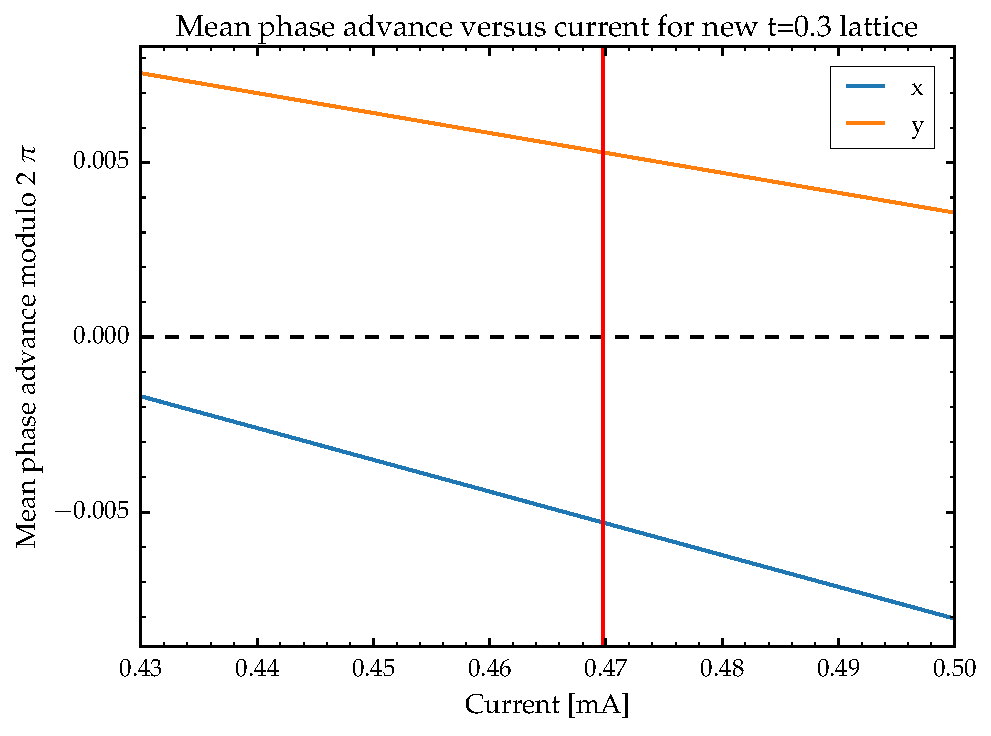
\includegraphics[width=\columnwidth]{adjusted_t0pt3phase.pdf}%
	\caption{\label{fig:phase_adjust} The operating current for an adjusted IOTA lattice is found by minimizing the deviation in the phase advance in each plane from zero.}
\end{figure}

This procedure was repeated to construct optimized lattice and beam configurations for each combination of tune-depression and $t$ value considered.


% Put \label in argument of \section for cross-referencing
%\section{\label{}}
\subsection{Simulation Results}
To examine the operation of the nonlinear element we start the simulation with a bunch 
that has been matched into the elliptic potential as previous described, but after the 
matching procedure the bunch centroid is displaced from zero in x by \SI{+100}{\mu m}. A 
comparison of bunch centroid motion with and without the noninear element is shown in 
Fig. \ref{fig:nll_on-off} With a purely linear lattice this displaced bunch exhibits coherent 
oscillations of the centroid around zero indefinitely. With the nonlinear element turned on 
these oscillations  rapidly damp due to the tune spread created by the nonlinear magnet. 

\begin{figure}
	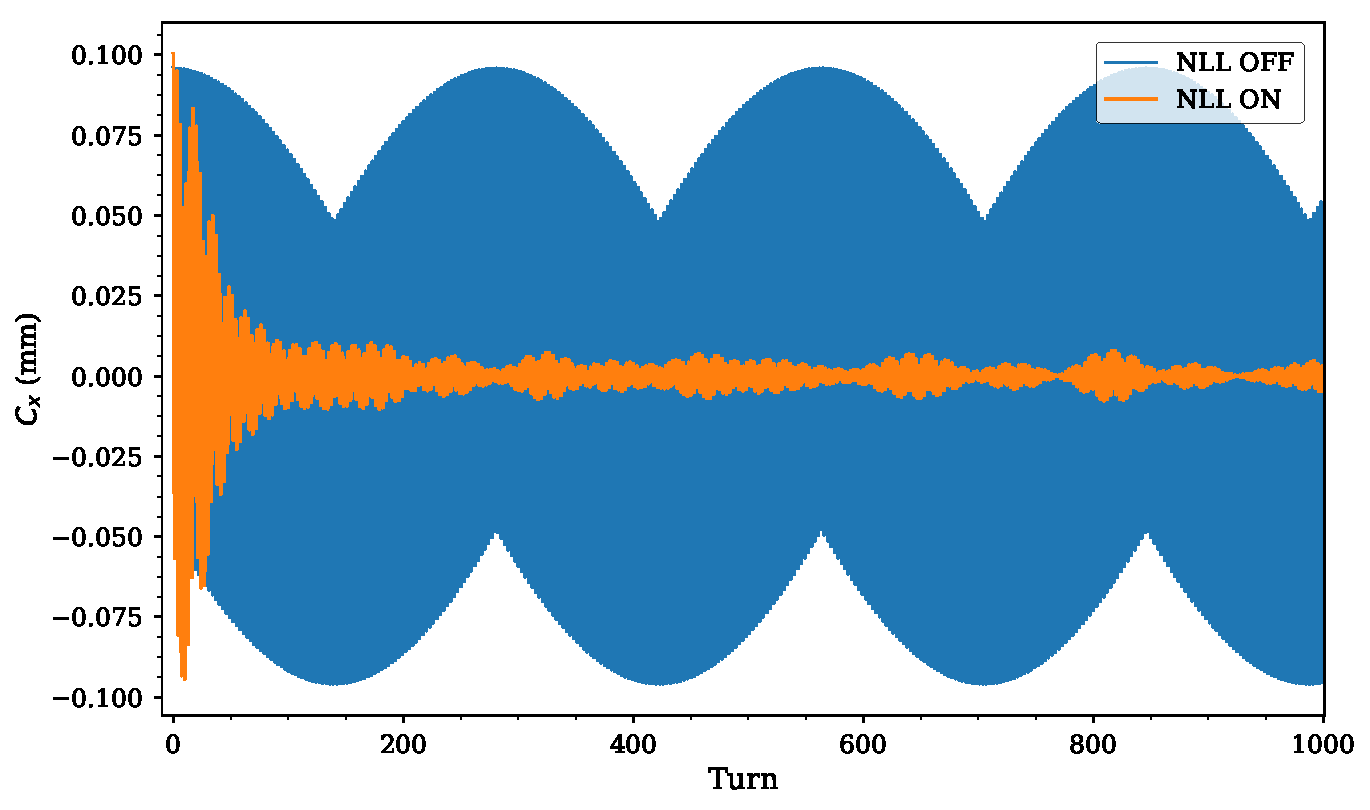
\includegraphics[width=\columnwidth]{t_on-off_8um.pdf}%
	\caption{\label{fig:nll_on-off} Centroid ($C_x$) motion for a matched bunch displaced 
	horizontally by \SI{100}{\mu m}. Motion with the nonlinear element off is shown in blue 
	and with nonlinear element on in orange. Space charge is not included in the 
	simulation.}
\end{figure}

The tune spread induced for the zero current case is shown in Fig. 
\ref{fig:zc_tune_spread}. Because the multipole expansion of the elliptic potential has a 
quadrupole term in the lowest order there is a splitting of the horizontal and vertical 
tunes, as well as the spread from the higher-order terms. 
%TODO: Remake simulation with ZC and t=0, currently only have SC case

\subsubsection{Nonlinear Decoherence with Space Charge}

We now illustrate what happens when space charge is included in the simulation. The 
space charge model used in Synergia was previously discussed. For all simulations with 
space charge a tune depression of $0.03 \times 2\pi$ $/$ turn is maintained. For a 
waterbag bunch distribution an asymmetric distribution of tunes, shifted from the lattice 
design point, occurs. To match the beam current to the ideal tune depression as closely 
as possible a scan over the current is performed. The ideal current is selected to that 
which maximizes the number of particles in the bunch that have a phase advance from the 
exit to the entrance of the nonlinear element within one standard deviation of zero. Values 
for various emittances are shown in Table. \ref{table:sc_params}.

\begin{table}
	\caption{\label{table:sc_params} Characteristics of the bunch and lattice for 
	simulations.}
	\begin{ruledtabular}
	\begin{tabular}{l|cc}
		\hline
		Quantity & Value & Units \\
		\hline
		\multicolumn{3}{c}{} \\[-1em]
		\multicolumn{3}{c}{Beam Parameters} \\
		\hline
		\\[-1em]
		$dQ_{SC}$ & 0.03 & - \\
		$\varepsilon_0$ & 4, 8, 12, 16& $mm-mrad$ \\
		$I$ &0.2056, 0.4113, 0.6169,  0.8225 & $mA$ \\
		K    &  2.5  & MeV \\
		$\Delta x$& 100 & $\mu m$ \\
		\hline
		\multicolumn{3}{c}{} \\[-1em]
		\multicolumn{3}{c}{Nonlinear Magnet Parameters} \\
		\hline
		\\[-1em]
		t & 0.2/0.4 & - \\
		c & 0.1 & $m^{1/2}$ \\
		$\psi_{nll}$& 0.3 & $2\pi$ \\
		\hline
	\end{tabular}
	\end{ruledtabular}
\end{table}	

For a bunch with an initial emittance of \SI{8}{mm-mrad} and with a nonlinear magnet 
strength $t=0.4$ the turn-to-turn centroid motion is shown in Fig. \ref{fig:sc_on-off}. It is 
seen that with space charge now included the damping time is greatly increased and one 
thousand turns is no longer sufficient to see the centroid motion decrease appreciably. 
The main culprit for this loss in effectiveness of nonlinear decoherence is the space 
charge induced tune spread. The assumption of time-invariance created by the ideal 
T-insert is broken for particles that do not maintain the design tune. 

\begin{figure}
	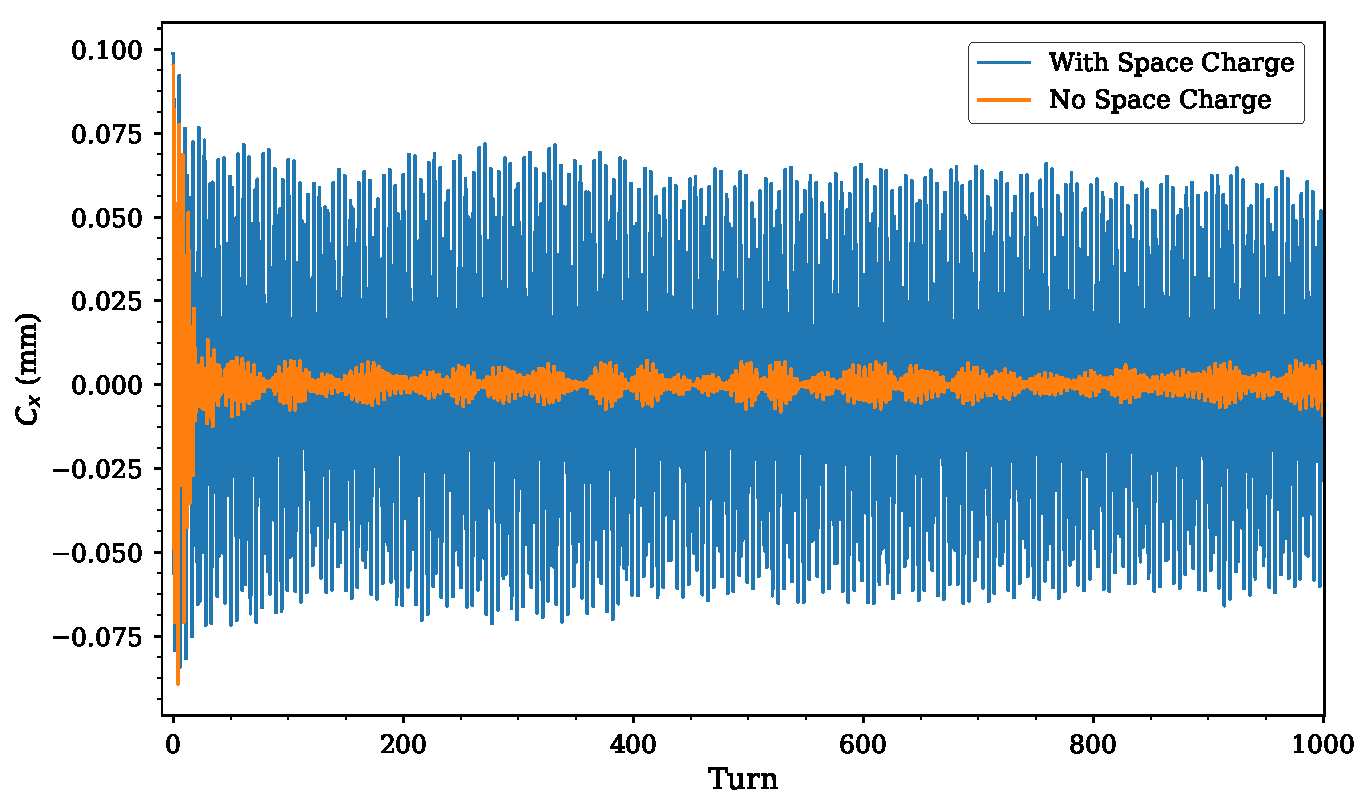
\includegraphics[width=\columnwidth]{sc-zc_centroid_motion_xoffset-100um.pdf}%
	\caption{\label{fig:sc_on-off} Centroid ($C_x$) motion for a matched bunch displaced 
		horizontally by \SI{100}{\mu m}. Only single particle dynamics are considered for the 
		simulation in orange. Space charge is included for the simulation shown in blue.}
\end{figure}

% Create the reference section using BibTeX:
\bibliography{hall}

\end{document}
%
% ****** End of file apstemplate.tex ******
